\documentclass[tikz,crop]{standalone}
\usepackage{tikz}
\usepackage{xcolor}
\usepackage{fontspec}

%\standaloneenv{tikzpicture}

\setmainfont{C059}
%/usr/share/fonts/gsfonts/C059-Roman.otf

\colorlet{bordercolor}{white} % for final version
%\colorlet{bordercolor}{black} % for debugging

%\definecolor{goldcolor}{cmyk}{0,17,55,50}
\definecolor{goldcolor}{RGB}{132, 117, 78}


\begin{document}
\noindent 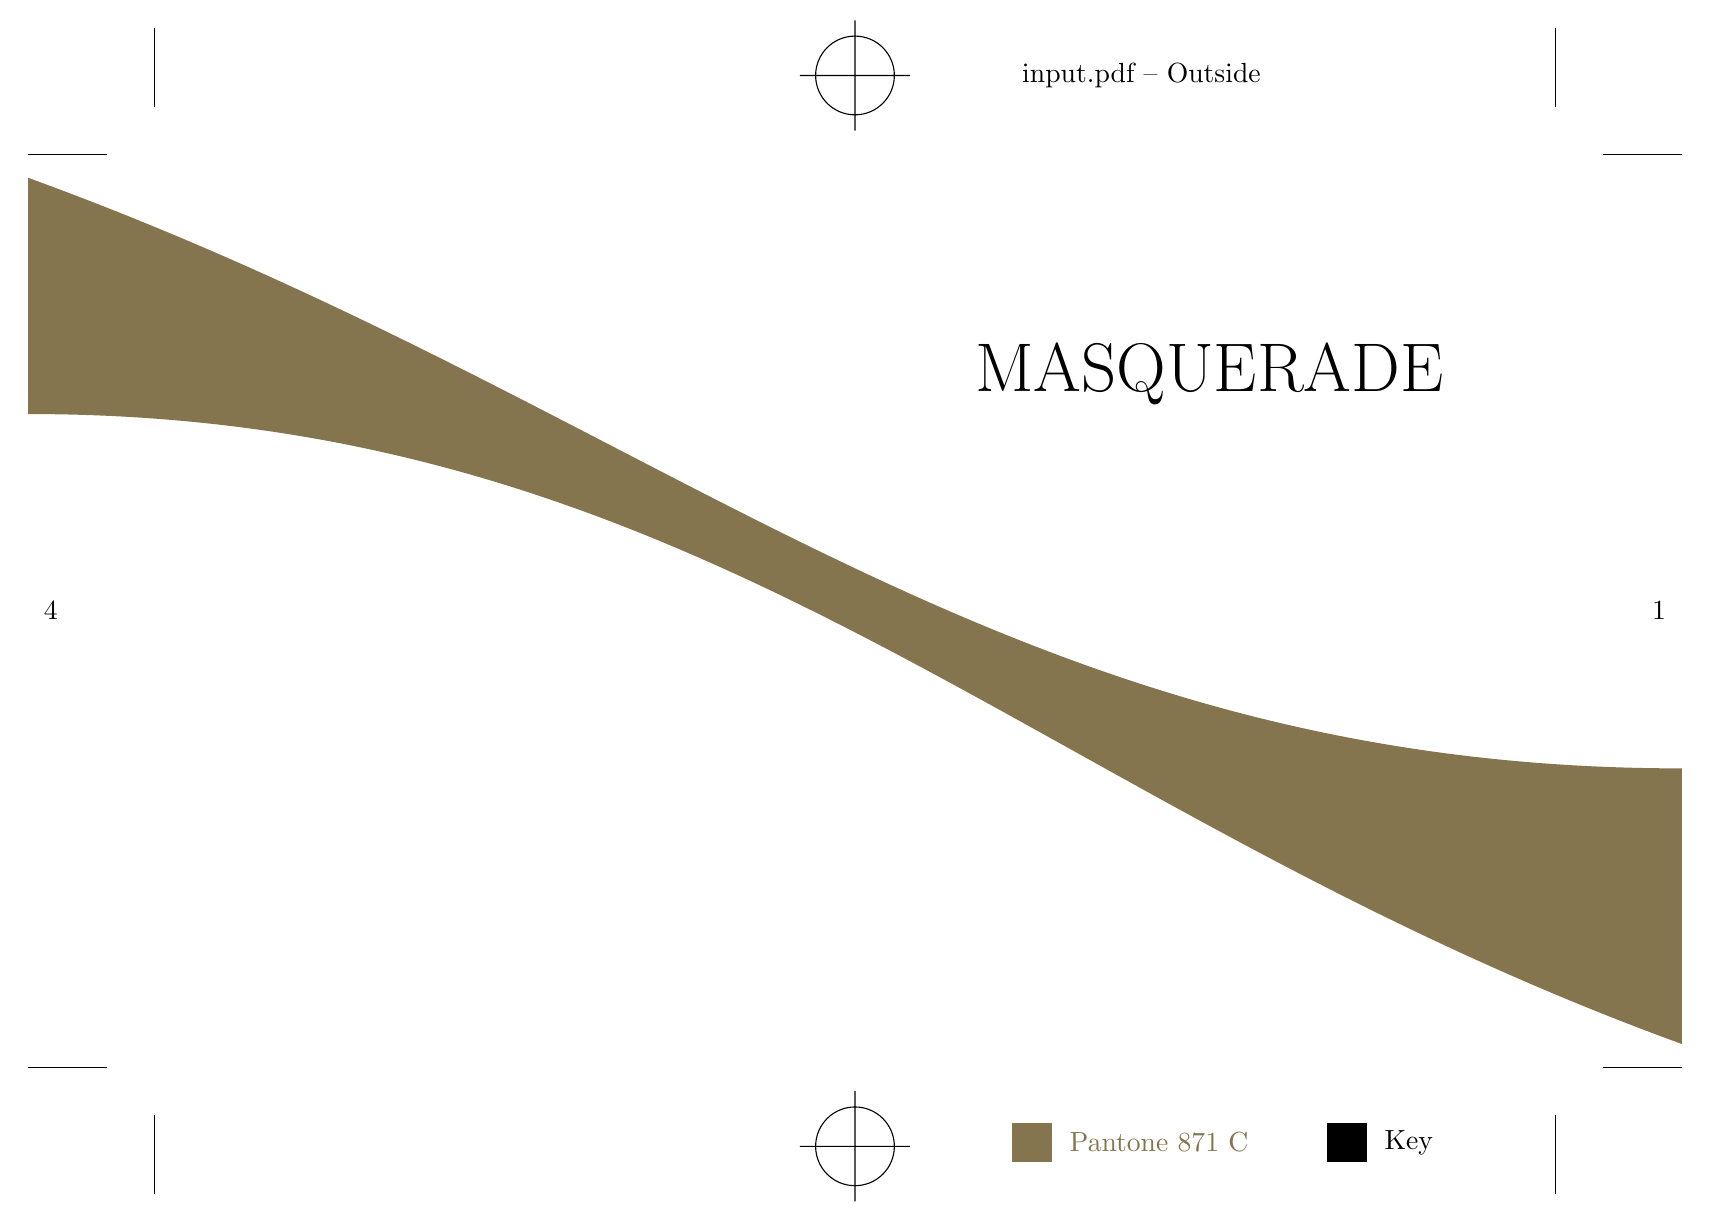
\begin{tikzpicture}[x=1mm, y=1mm]
        \useasboundingbox[draw=bordercolor] (-105, -74) rectangle (105, 74); % A5 paper -> A6 booklet

        % Coca cola sash
        \fill[goldcolor] (-105, 55) to[out=-20,in=180] (105, -20) -- (105, -55) to[out=160, in=0] (-105, 25) -- cycle;

        \node at (45,30) {\Huge MASQUERADE};

        % Printer's marks {{{
        \draw (0, 68) circle(5) +(0:-7) -- +(0:7) +(90:-7) -- +(90:7); % Center mark
        \draw (0, -68) circle(5) +(0:-7) -- +(0:7) +(90:-7) -- +(90:7); % Center mark
        \draw  % Crop marks
                (-105, 58) -- (-95, 58) (105, 58) -- (95, 58) %
                (-105, -58) -- (-95, -58) (105, -58) -- (95, -58) %
                (-89, 74) -- (-89, 64) (89, 74) -- (89, 64) %
                (-89, -74) -- (-89, -64) (89, -74) -- (89, -64) %
                ;
                \node[anchor=west] at (20,68) {\jobname.pdf -- Outside};
                \node[anchor=west] at (100,0) {1};
                \node[anchor=east] at (-100,0) {4};
                \fill[goldcolor] (20, -65) rectangle +(5, -5) node[midway, right]{\hspace{1em}Pantone 871 C};
                \fill[black] (60, -65) rectangle +(5, -5) node[midway, right]{\hspace{1em}Key};
        % }}}
\end{tikzpicture}

\noindent\begin{tikzpicture}[x=1mm, y=1mm]
        \useasboundingbox[draw=bordercolor] (-105, -74) rectangle (105, 74); % A5 paper -> A6 booklet
        % Printer's marks {{{
        \draw (0, 68) circle(5) +(0:-7) -- +(0:7) +(90:-7) -- +(90:7); % Center mark
        \draw (0, -68) circle(5) +(0:-7) -- +(0:7) +(90:-7) -- +(90:7); % Center mark
        \draw  % Crop marks
                (-105, 58) -- (-95, 58) (105, 58) -- (95, 58) %
                (-105, -58) -- (-95, -58) (105, -58) -- (95, -58) %
                (-89, 74) -- (-89, 64) (89, 74) -- (89, 64) %
                (-89, -74) -- (-89, -64) (89, -74) -- (89, -64) %
                ;
                \node[anchor=west] at (20,68) {\jobname.pdf -- Inside};
                \node[anchor=west] at (100,0) {3};
                \node[anchor=east] at (-100,0) {2};
                \fill[goldcolor] (20, -65) rectangle +(5, -5) node[midway, right]{\hspace{1em}Pantone 871 C};
                \fill[black] (60, -65) rectangle +(5, -5) node[midway, right]{\hspace{1em}Key};
        % }}}
\end{tikzpicture}

\end{document}
